\subsection{Estimation of the Tau Leptons}
\label{sect:tau}
Tau leptons can decay hadronically and appear as a thin jet and enter the hadronic searches. 
To estimate the contamination from such events a method similar to what is used for the lost lepton background is used here. The number of 
events with exactly one real tau is corrected by accounting for the reconstruction and acceptance efficiencies. In the other words:
\begin{linenomath}
\begin{equation}
	N_{W\rightarrow{\tau\nu}} = \frac{N_{\tau}^{reco} - N_{\tau}^{bg}}{\varepsilon_{\tau}},
	\label{eq:TauEstimation}
\end{equation}
\end{linenomath}
where $N_{\tau}^{reco}$ is the number of events with one reconstructed tau, $N_{\tau}^{bg}$ is the number of events with a 
fake tau and $\varepsilon_{\tau}$ denotes the probability for a generated
$W \rightarrow \tau\nu, \ \tau \to had$ event passing the selection cuts to have a reconstructed and identified tau. 
The efficiency $\varepsilon_{\tau}$ is extracted from simulation. In average, $\varepsilon_{\tau}$ is found to be $\sim24$\%. 5\% systematic 
uncertainty is assigned to this value to take into account the differences between data and MC.
The transverse mass (\mt) of the system of the reconstructed tau and MET is forced to be less than 100 GeV/$c^2$ to decrease 
the signal contamination.  The number of events with a fake tau, $N_{\tau}^{bg}$ is found from the MC simulation and a 50\% systematic 
uncertainty is assigned to this value.

The \mttwo distribution of the events with all selection cuts which have an
identified tau in the final state is shown in Figure \ref{fig:MT2Tau}.
\begin{figure}[!htb]
\centering
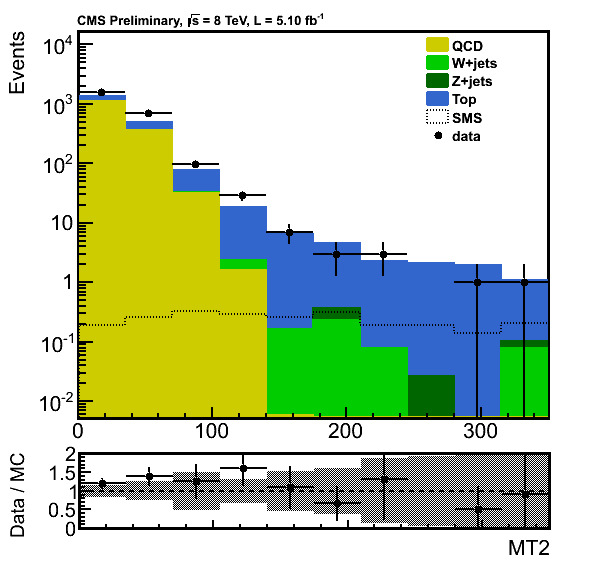
\includegraphics[width=0.49\textwidth]{figs/MT2Tau.png}
\caption{\mttwo distribution for events with at least one tau in data and MC with all selection cuts.}
\label{fig:MT2Tau}
\end{figure}
Scale factors of the tau selection are not applied and it can be the source of the discrepancies between data and MC. 
In Table~\ref{table:Tau_yield} 
\begin{table}[!htb]
\begin{center}
\small
\begin{tabular}{lcccccc}
\hline\hline
\mttwo (GeV)   &  QCD   & Z+Jets & W+Jets & Top & MC(sum) & data \\
\hline
 full range & 1480.06 & 0.35 & 9.59 & 417.80 & 1907.79 $\pm$ 182.88 & 2309.00\\
$125-\infty$ &   1.46 & 0.08 & 0.94 &  20.13 &   22.61 $\pm$ 4.57   & 21.00\\
\hline\hline
\multicolumn{7}{c}{cut on \mindphifour is relaxed}\\
\hline\hline
$125-\infty$ &      6.21 & 0.11 & 2.03 & 31.91 & 40.25 $\pm$ 6.18 & 34.00\\
\hline\hline
\end{tabular}
\caption{MC and data event yields in full range and signal region. The last row shows the yields after relaxing the cut.
The error on the total background is purely statistical.}
\label{table:Tau_yield}
\end{center}
\end{table}
contribution of different samples in the plot of Figure \ref{fig:MT2Tau} is shown. It can be seen that the statistics in the signal
region is poor. To decrease the uncertainties of the predictions, the cut on  \mindphifour is relaxed. 
The last row of the table shows the statistics after this relaxation. The scale factor to compensate this relaxation is 
read from MC.

Table \ref{table:MT2TauCutsRelaxed} 
\begin{table}[!htb]
\begin{center}
\small
\begin{tabular}{lccc}
\hline\hline
  \mttwo bin  &      MC Truth     &         Prediction in MC       & Prediction in Data \\\hline
$125-\infty$   &  78.40 $\pm$ 9.64 &  77.38 $\pm$ 19.94 $\pm$ 35.63 & 57.20 $\pm$ 18.83 $\pm$ 33.00\\
\hline\hline
\end{tabular}
\caption{Prediction of the tau contamination in the signal region in both data and MC.}
\label{table:MT2TauCutsRelaxed}
\end{center}
\end{table}
shows the performance of the method on MC and data. The quoted uncertainties of the predictions are statistical and systematical, respectively.
